\par
\section[Erdbebenerkennung unter Android (Christopher Althaus)]{Erdbebenerkennung unter Android\begin{tiny} (Christopher Althaus)\end{tiny}}
Die Erdbebenerkennung innerhalb von Android ist ein wesentlicher Bestandteil des gesamten Systems. Die Realisierung folgt dabei im wesentlichen zwei Grundprinzipien. Zum einen soll die Empfindlichkeit bewusst hoch sein, zum anderen soll der Akkuverbrauch so gering wie möglich gehalten werden.\\
Die hohe Empfindlichkeit ist darin begründet, dass es besser ist einen Fehlalarm auszulösen, als ein reales Erdbeben nicht als solches zu erkennen. Der möglichst geringe Akkuverbrauch ist der Benutzerakzeptanz der Anwendung zuzuschreiben. Kein Anwender möchte eine Software installieren, welche den Akku in kürzester Zeit leert. Um den Akkuverbrauch gering zu halten, bedarf es somit eines möglichst einfach aufgebautem Erkennungsalgorithmus für Erdbeben.
\subsection{Abfragen der Sensordaten unter Android}
Innerhalb der Android Anwendung werden die Sensordaten in einem Service im Hintergrund ab-gefragt. Dieser Service nutzt dazu den sogenannten \textit{SensorManager} aus dem \textit{android.hardware} Paket. Mittels des \textit{SensorManagers} ist es möglich, auf alle Sensoren eines Android Gerätes zuzugreifen. Daraufhin wird ein neuer Sensor vom Typ \textit{Accelerometer} angelegt, welcher daraufhin im \textit{SensorManager} registriert werden kann. Im Listing \ref{lst:AccelCollect} ist der dafür nötige Code aufgeführt.
\begin{lstlisting}[caption={Abfragen der Sensordaten unter Android},label=lst:AccelCollect]
public final String ACCEL_SAMPLE = "com.th.nuernberg.quakedetec.ACCEL_SAMPLE";
public final String ACCEL_SAMPLE_KEY = "ACCELERATION_SAMPLE";
SensorManager sensManager = getSystemService(Context.SENSOR_SERVICE);
Sensor accel = sensManager.getDefaultSensor(Sensor.TYPE_ACCELEROMETER);
sensManager.registerListener(sensListener, accel, SensorManager.SENSOR_DELAY_UI);

private final SensorEventListener sensListener = new SensorEventListener() {
	public void onSensorChanged(SensorEvent e) {
		float x = e.values[0]; 
		float y = e.values[1]; 
		float z = e.values[2]; 
		long t = System.currentTimeMillis();
		AccelSample accelSample = new AccelSample(x, y, z, t);
		broadcastSingleSample(accelSample);
	}
};


protected void broadcastSingleSample(AccelSample sample) {
	Intent intent = new Intent(ACCEL_SAMPLE);
	intent.putExtra(ACCEL_SAMPLE_KEY, (Parcelable) sample);
	sendBroadcast(intent);
}
\end{lstlisting}
Zunächst wird, wie bereits geschrieben, der \textit{SensorManager} und die Variable accel vom Typ \textit{Sensor} als Beschleunigungssensor initialisiert. Daraufhin wird mittels des \textit{SensorManagers} ein \textit{SensorEventListener} namens \textit{sensListener} für den angelegten Beschleunigungssensor registriert. Dieser \textit{SensorEventListener} wird daraufhin bei jedem Event des Beschleunigungssensor aufgerufen. Beim Registrieren des Sensors wird zudem die Aktualisierungsrate mit angegeben. Diese ist momentan auf den Wert \textit{SENSOR\_DELAY\_UI} eingestellt, was einer eher mittleren Aktualisierungsrate entspricht. Würde die Rate jedoch höher gesetzt werden, würde dies den Akkuverbrauch in die Höhe treiben. Die nächst niedrigere Stufe wäre \textit{SENSOR\_DELAY\_NORMAL}. Sie wird innerhalb von Android zur Displayausrichtung genutzt und hat somit eine zu langsame Aktualisierungsrate, dass sie zur Erkennung von Erdbeben nicht geeignet wäre.\\
Im \textit{SensorEventListener} werden nun die aktuellen Sensorwerte entgegengenommen. Dabei handelt es sich um die Beschleunigungswerte der X-, Y- und Z-Achse. Die Sensordaten werden nun zusammen mit der aktuellen Systemzeit in einer Variable vom Typ \textit{AccelSample} gespeichert. Diese Klasse dient lediglich dazu, die Sensordaten eines Zeitpunktes innerhalb des Systems mittels eines Broadcasts zu verbreiten. Dieser Broadcast wird von der Methode \textit{broadcastSingleSample} ausgelöst.\\
Prinzipiell könnte auch innerhalb des \textit{SensorEventListeners} die Auswertung der Beschleunigungssensordaten stattfinden. Da jedoch neben der Erdbebenerkennung auch das Diagramm, welches der Nutzer innerhalb der App sieht, diese Daten benötigt, ist es der übliche Weg, einmal innerhalb einer Applikation die Daten vom Sensor anzufragen und daraufhin innerhalb der Anwendung diese Daten mittels eines Broadcast zu verteilen.\\
Wie in der Implementierung der \textit{broadcastSingleSample} Methode zu sehen, wird innerhalb dieser Methode ein Intent angelegt. Intents werden vom Android Betriebssystem für den asynchronen Austausch von Nachrichten verwendet. Dem angelegten Intent wird dabei der String \textit{ACCEL\_SAMPLE} als Argument übergeben. Hierbei handelt es sich um eine Art Schlüssel für die auszuführende Aktion des Intents, welcher später dazu benutzt werden kann, Intents dieses Schlüssels abzufangen und zu verwenden. Ebenso werden dem Intent die Beschleunigungssensordaten angehangen. Dies geschieht mittels einer Key/Value Angabe. Dabei ist der String \textit{ACCEL\_SAMPLE\_KEY} der Schlüssel für die übergebenen Beschleunigungssensordaten der Variable sample. Mittels des hier angegebenen Schlüssels können Empfänger dieses Intents, die Daten, welche ihm hinzugefügt worden sind, zweifelsfrei zuordnen. Zum Ende der Methode wird das Intent als Broadcast verschickt.\\
Möchte nun eine Activity oder ein anderer Service auf die Daten des Intents zugreifen, wird ein Broadcast-Receiver benötigt, welcher auf Intents mit dem Schlüssel aus der Variable \textit{ACCEL\_SAMPLE} wartet. Eine beispielhafte Implementierung eines solchen Broadcast-Receivers ist dabei im nachfolgenden Listing \ref{lst:AccelReceiver} dargestellt.
\begin{lstlisting}[caption={Broadcast-Receiver zum Auslesen der Beschleunigungssensordaten},label=lst:AccelReceiver]
private class AccelerationBroadcastReceiver extends BroadcastReceiver {
	@Override
	public void onReceive(Context context, Intent intent) {
		if (intent.getAction().equals(Accelerometer.ACCEL_SAMPLE)) {
			AccelSample sample = intent.getParcelableExtra(Accelerometer.ACCEL_SAMPLE_KEY);
			if (sample != null) {
			//Erdbebenauswertung
			}
		}
	}
}
\end{lstlisting}
Wie im Quellcodeauszug ersichtlich, empfängt ein Broadcast-Receiver zunächst jegliche auftretende Intents. Jedoch kann unter der Verwendung des Schlüssels, welcher dem Intent zugewiesen worden ist, jedes eingehende Intent dahingehend überprüft werden, ob es sich um das gefragte Intent handelt oder nicht. Ist dies der Fall, so können die dem Intent angehangenen Daten ausgelesen werden. Hierzu wird der Schlüssel verwendet, welcher dem angehangenen Inhalt zugewiesen worden ist. In diesem Fall also der Wert von \textit{ACCEL\_SAMPLE\_KEY}, der Klasse \textit{Accelerometer}.
Mit dem ausgelesenen Wert des Intents stehen nun im Broadcast-Receiver die Beschleunigungswerte eines einzelnen Zeitpunktes zur Verfügung. Somit können diese für die Erdbebenauswertung genutzt werden, welche im folgenden erläutert werden soll.

\subsection{Erdbebenauswertung}
Wie bereits erwähnt, soll der zur Auswertung benutzte Algorithmus möglichst ressourcenschonend implementiert werden. Deshalb ist gleich zu Beginn der Implementierung beschlossen worden, dass die Erkennung nicht alle drei Achsen (X, Y, Z) auswerten soll, sondern den Betrag aller Beschleunigungen.\\
Prinzipiell kann man sich die vom Beschleunigungssensor erhaltenen Werte als Vektoren
vorstellen, welche einen rechtwinkligen Raum aufspannen. Möchte man nun den Betragswert dieser Vektoren bestimmen, genügt es, die Raumdiagonale $r$ dieses Raumes zu berechnen. Diese kann
mit der Formel $|r| = \sqrt{x^2 + y^2 + z^2}$ berechnet werden. Die Formel beruht dabei auf dem Satz des Pythagoras. Zunächst wird dabei die Diagonale der Grundfläche, welche durch zwei Achsen
aufgespannt wird, berechnet ($d = \sqrt{x^2 + y^2}$). Daraufhin wird der Satz des Pythagoras ein erneutes Mal auf die verbleibende Achse angewendet ( $|r| = \sqrt{d^2 + z^2}$). Durch das Quadrieren von $d$ fällt dessen Wurzel weg, womit sich die oben genannte Formel ergibt.\\
Da auf der Erde stets eine Erdanziehungskraft von etwa 9,81 $\frac{m}{s^2}$ wirkt, liegt der berechnete Betragswert der Beschleunigung bei einem still liegendem Gerät stets bei etwa 9,81 $\frac{m}{s^2}$. Um die Erkennung von Beschleunigungsänderungen zu vereinfachen, ist deshalb entschieden worden, die Erdbeschleunigung vom Betragswert abzuziehen. Auf diese Weise ergibt sich letztendlich die Formel $|a| = \sqrt{x^2 + y^2 + z^2} - 9,81 \frac{m}{s^2}$ zur Berechnung der betragsmäßigen Beschleunigung des Gerätes. Wird nun das Gerät bewegt, ergeben sich Ausschläge um den Nullpunkt herum, wie in Abbildung \ref{fig:accelnormal} dargestellt.

\begin{figure}[H]
\centering
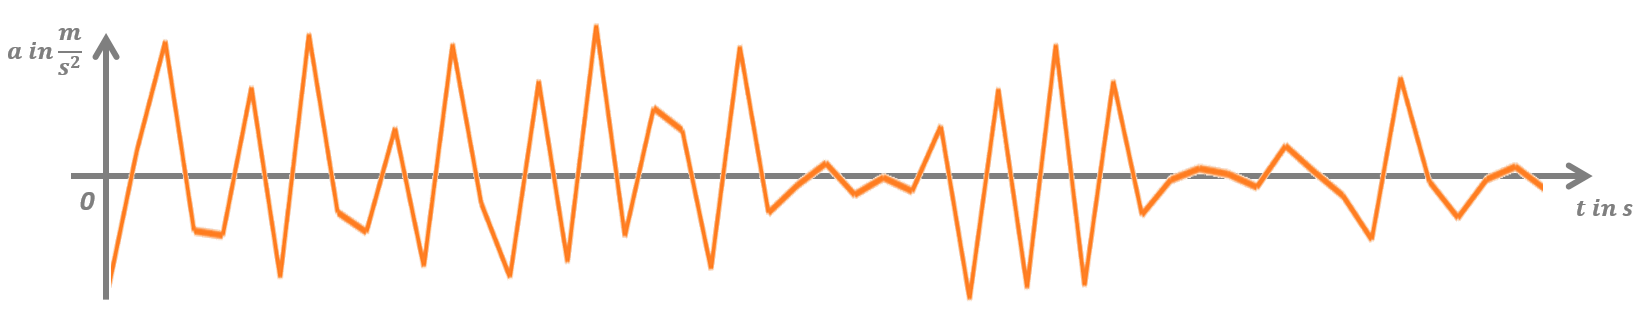
\includegraphics[width=\textwidth]{/accelnormal.png}
\caption{Beschleunigungssignal nach der Zusammenfassung}
\label{fig:accelnormal}
\end{figure}
Die dargestellten Ausschläge sind eine Aufzeichnung des Beschleunigungssignals, während das Gerät mit erdbebenartigen Schlägen bewegt worden ist. Durch die Rüttelbewegung des Gerätes wirkt darauf abwechselnd eine Beschleunigung in Richtung der Erdanziehung, wodurch ein positiver Ausschlag entsteht und daraufhin eine Beschleunigung entgegengesetzt der Erdanziehung. Dadurch wird die Erdanziehung aufgehoben und es entsteht ein negativer Ausschlag.\\
Da bei Erdbeben in kurzer Zeit eine hohe Anzahl von Schlägen auf das Gerät einwirken, ist es in Anbetracht dieser Tatsachen möglich, das Beschleunigungssignal mittels der Zählung von Nulldurchläufen des Signals auf erdbebenartige Schläge hin zu untersuchen.\\
Durch die Empfindlichkeit des Beschleunigungssensor sind jedoch auch in einer absoluten Ruheposition des Gerätes stets Nulldurchläufe des Signals messbar. Daher ist es notwendig, erst Signalwerte, die über einem gewissen Schwellwert liegen, als Nulldurchläufe zu zählen.
Dieser Umstand soll in der folgenden Abbildung \ref{fig:accellines} verdeutlicht werden.

\begin{figure}[H]
\centering
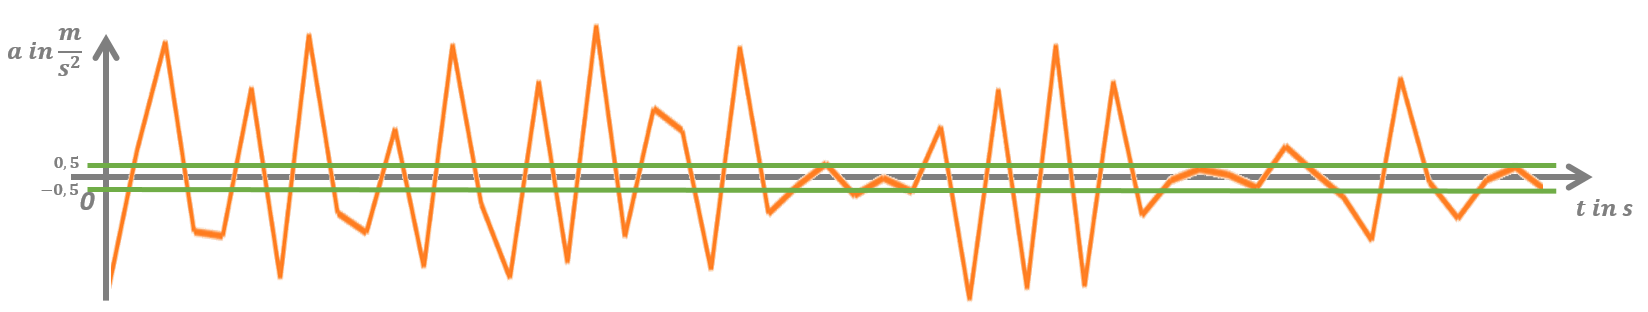
\includegraphics[width=\textwidth]{/accellines.png}
\caption{Beschleunigungssignal mit Schwellwerten}
\label{fig:accellines}
\end{figure}
Die grünen Linien innerhalb des Diagramms sind dabei die definierten Schwellwerte. Hierzu ist in der Implementierung ein Wert von +/- 0,5 $\frac{m}{s^2}$ gewählt worden. Wie im Diagramm ersichtlich,
stellt dieser Schwellwert bei wahrnehmbaren Erschütterungen keinerlei Einschränkung dar und filtert zuverlässig kleinere Signalstörungen heraus.\\
Die eigentliche Erkennung von Erdbeben gestaltet sich nun denkbar einfach und somit auch ressourcenschonend. Für die eigentliche Signalanalysierung werden lediglich zwei Variablen benötigt. Eine Variable legt dabei fest, ob der letzte Signalwert positiv oder negativ war. Die zweite Variable wird bei jedem Signalwechsel von positiv auf negativ erhöht. Betrachtet man diese Auswertemethode anhand des verwendeten Signalverlaufs der vorherigen Abbildungen, so ergibt sich ein Auswerteergebnis, welches in Abbildung \ref{fig:accelmarked} dargestellt ist.
\begin{figure}[H]
\centering
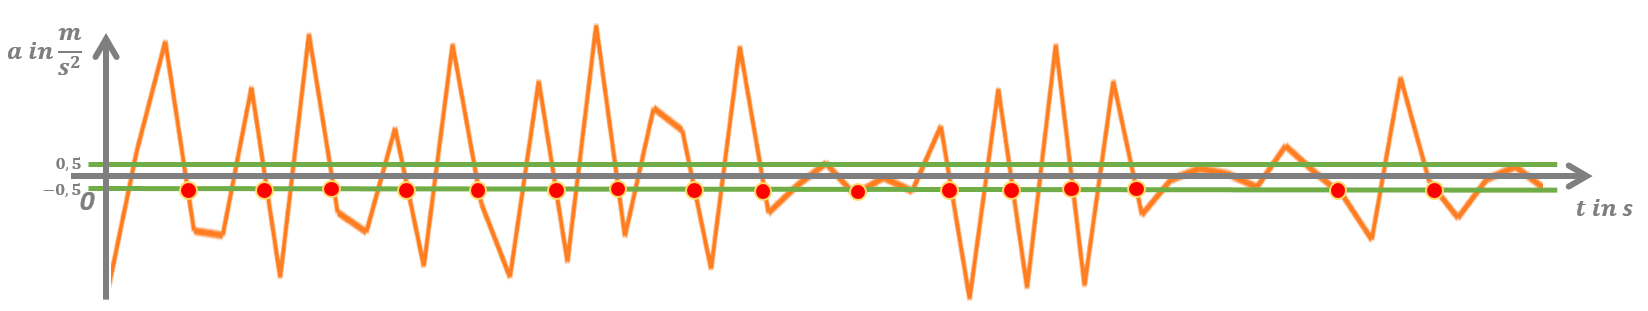
\includegraphics[width=\textwidth]{/accelmarked.png}
\caption{Beschleunigungssignal mit Nulldurchläufen analysiert}
\label{fig:accelmarked}
\end{figure}
Jede rote Markierung des Signals steht hierbei für einen Signalwechsel. Wie ersichtlich, ergibt sich somit für jeden einzelnen Ausschlag eine Markierung. Zum Ende des Signals wird dabei auch die Filterung mittels der Schwellwerte deutlich. Hier erreicht ein Signalwechsel diesen Schwellwert nicht und wird deshalb auch nicht mitgezählt.\\
Zur Erkennung von Erdbeben wird nun in einem bestimmten Zeitrahmen die Anzahl dieser Signalwechsel gezählt. In der momentanen Implementierung wird dazu ein Zeitraum von fünf Sekunden ausgelöst.\\
Nachfolgend soll die Implementierung in Java erläutert werden. Im Listing \ref{lst:AccelGlobalVals} sind hierzu die benötigten globalen Variablen aufgeführt.
\begin{lstlisting}[caption={Globale Variablen der Erbebenerkennung},label=lst:AccelGlobalVals]
private boolean signalGreaterZero = true;
private int signalChangeCount = 0;
private long analyseTimeSpan = System.currentTimeMillis(); 
private int accelFreq = 0;
\end{lstlisting}
Die Variable \textit{signalGreaterZero} speichert jeweils für den letzten Signalwert, ob dieser positiv oder negativ war. Die Variable \textit{signalChangeCount} ist für die Zählung der Signalwechsel verantwortlich. In der Variable \textit{analyseTimeSpan} dient zur Speicherung der Systemzeit, um alle fünf Sekunden eine Auswertung zu machen. Die Variable \textit{acceFreq} dient dem Auswerten der Frequenz des Beschleunigungssensor. Dieser Umstand wird nachfolgend noch genauer erläutert.\\
Anschließend soll die eigentliche Signalauswertung erklärt werden. Dazu ist zunächst, wie bereits beschrieben, die Zählung der Signalwechsel nötig. Die dafür notwendige Implementierung ist im nachfolgendem Listing \ref{lst:AccelCount} aufgeführt.
\begin{lstlisting}[caption={Implementierung der Erdbebenerkennung},label=lst:AccelCount]
AccelSample sample = intent.getParcelableExtra(Accelerometer.ACCEL_SAMPLE_KEY); 
	if (sample != null) {
		if (sample.abs < -0.5 && signalGreaterZero) {
			signalChangeCount++;
			signalGreaterZero = false; 
		} else if (sample.abs > 0.5)
			signalGreaterZero = true;
	...
}
\end{lstlisting}
Wie im Auszug ersichtlich, ist die Zählung der Signalwechsel mittels des Beschleunigungssensorwertes aus dem Intent des bereits beschriebenen Broadcast-Receivers implementiert. In der Abfrage wird zunächst überprüft, ob der Wert des Sensors größer ist, als der vorgegebene Schwellwert von +/- 0.5 $\frac{m}{s^2}$. Ist dies der Fall, wird überprüft ob ein Vorzeichenwechsel des Signals stattgefunden hat. Ist dies der Fall, wird beim Vorzeichenwechsel von positiv zu negativ die Variable \textit{signalChangeCounter} erhöht und das neue Vorzeichen mittels der Variable \textit{signalGreaterZero} gespeichert. Nachdem nun die Nulldurchläufe gezählt werden, wird eine Auswertung der gezählten Durchläufe in einem bestimmten Zeitrahmen benötigt. Diese wird im nachfolgenden Listing \ref{lst:AccelDetect} erläutert.
\begin{lstlisting}[caption={Analyse der gezählten Nulldurchläufe},label=lst:AccelDetect]
if (System.currentTimeMillis() - analyseTimeSpan> 5000) {
	double alarmRatio = 0;
	if(signalChangeCount != 0)
		alarmRatio = (double)signalChangeCount/(double)accelFreq * 100.0;
	//Alarmauswertung abhaenig von der Frequenz
	double alarmFrequRel = accelFreq * 0.01 + 0.5;
	alarmRatio = alarmRatio * alarmFrequRel;
							
	if (alarmRatio > 25) 
		sendAlarmToServer();
							
	analyseTimeSpan = System.currentTimeMillis();
	accelFreq = 0;
	signalChangeCount = 0;
}
accelFreq++;
\end{lstlisting}
Die Analyse der gezählten Signalwechsel wird dabei alle fünf Sekunden ausgeführt. Dazu wird die Variable \textit{analyseTimeSpan}, welche den Zeitpunkt der letzten Analyse abspeichert, bei jedem Aufruf des Broadcast-Receivers mit der aktuellen Systemzeit verglichen. Nachdem eine Zeitspanne von über fünf Sekunden vergangen ist, wird die Analyse gestartet.\\
Wie ersichtlich, reicht es nicht aus, lediglich die Anzahl der gezählten Spitzen zur Auswertung heranzuziehen. Das liegt daran, dass der Sensor innerhalb von Android keine gleichbleibende Frequenz besitzt und sich zudem die Frequenz von Gerät zu Gerät massiv unterscheiden kann. Die Frequenz der Sensoren reicht dabei von 2 Hz bis hin zu 50 Hz. Da bei einer Frequenz von 2 Hz innerhalb von fünf Sekunden lediglich 10 Messwerte verfügbar sind, ist hier eine zuverlässige Erkennung kaum möglich. Für die Auswertung wird deshalb eine Frequenz von 10 Hz als optimal angesehen und Frequenzen, die darüber oder darunter liegen dementsprechend mittels der Berechnung der Variable \textit{alarmFrequRel} angepasst. Die Auswahl der Frequenz von 10 Hz als Referenz begründet sich vor allem dadurch, dass sich während der Implementierung herausgestellt hat, dass die meisten Geräte den Beschleunigungssensor durchschnittlich mit dieser Frequenz aktualisieren. Anhand dieser Referenzfrequenz ist definiert worden, dass ab einem Verhältnis der gemessenen Signalwechsel zu den gesamten gemessenen Werten von größer 25\% ein Alarm ausgelöst werden soll. Da bei einer höheren Frequenz die Messwerte eines einzelnen Signalwechsels deutlich zunehmen, muss hier die Gewichtung von gemessenen Signalwechseln zu gemessenen Messwerten erhöht werden. Ist die Frequenz langsamer als 10 Hz, wird die Gewichtung der Signalwechsel dementsprechend reduziert. Ist die Variable \textit{alarmRatio} größer als 25, wird mittels der Methode \textit{sendAlarmToServer} ein Alarm an den Server geschickt. Nach der Auswertung werden alle zählenden Variablen wieder zurückgesetzt und der Zeitpunkt der Analyse in der Variable \textit{analyseTimeSpan} vermerkt, um nach fünf Sekunden erneut eine Analyse starten zu können.\\
Insgesamt sind die Parameter der Analyse während der Testphase stets angepasst worden und lösen nun bei allen zur Verfügung stehenden Testgeräten mit einer annähernd gleichen Empfindlichkeit einen Alarm aus.
\newpage